

We describe here the simplex algorithm as a method to solve linear
programs of the form $\max\{c^Tx \colon x \in \setR^n, \, Ax\leq b\}$ for some $A
\in \setR^{m\times n}$, $b \in \setR^m$ and $c \in \setR^n$. We assume first that the
matrix $A$ has full column rank, meaing that the columns of $A$ are
linearly independent.

\section{Halfspaces and the highest point problem}
\label{sec:two-variable-linear}



Throughout this chapter, we assume that the matrix $A \in \setR^{m\times n}$
defining our linear program $\max\{c^Tx \colon x \in \setR^n, Ax\leq b\}$ has
full column rank. We use the following notation.  For an index set
$I=\{i_1,\ldots,i_k\}\subseteq\{1,\ldots,m\}$, with $i_1<i_2<\cdots<i_k$, $A_I$ denotes
the $k\times n$ matrix whose $j$-th row is $a_{i_j}$, $j=1,\ldots,k$. Similarly
$b_I\in \setR^k$ denotes the vector whose $j$-th component is $b(i_j)$, $j=1,\ldots,k$. 

\begin{definition}[Basis, roof]
  \label{def:6}
  A \emph{basis}, or pictorially a \emph{roof} of a linear program
  $\max\{c^Tx \colon x \in \setR^n, \, Ax\leq b\}$ is an index set $\er
  \subseteq\{1,\ldots,m\}$ of cardinality $|\er| = n$ such that the matrix
  $A_\er\in \setR^{n\times n}$ is non-singular and the linear program
  $\max\{c^Tx \colon x \in \setR^n,\,  A_\er x\leq b_\er\}$ is bounded. The roof
  is degenerate, if this linear program
  $\max\{c^Tx\colon x\in\setR^n,\,A_\er x\leq b_\er\}$  has more than one optimal
  solution, otherwise, the roof is called non-degenerate. 
\end{definition}


%\begin{definition}[Halfspace]
%  \label{def:1}
%  A \emph{Halfspace} is a set of the form $ \{x \in \setR^n \mid a^Tx\leq\beta\}$,
%  where $a \in \setR^n$ 
%  and $\beta \in \setR$. We often write $a^Tx\leq\beta$ for the set $\{x \in \setR^n \mid a^Tx\leq\beta\}$. 
% The number $n$ is the \emph{dimension} of the halfspace.  The vector
% $a \in \setR^n$ is called the \emph{normal-vector} of the halfspace. 
% A point $x^* \in \setR^n$ \emph{satisfies} $a^Tx\leq\beta$ if $a^Tx^* \leq\beta$. The
% point $x^*$ \emph{violates} $a^Tx\leq\beta$ if $a^Tx^* > \beta$.
%\end{definition}

%\begin{figure}[htbp]
%  \centering
%  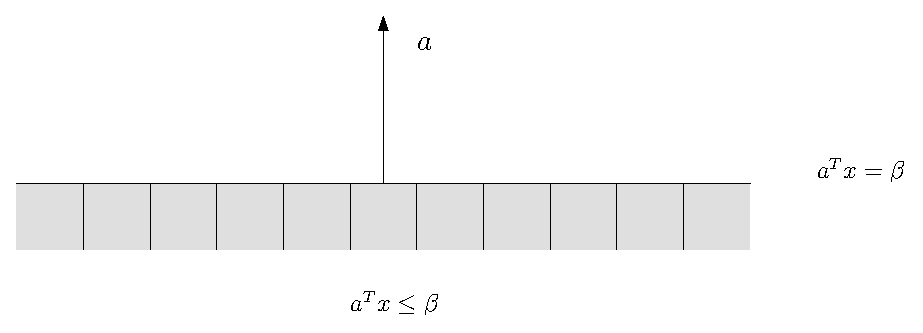
\epsfig{file=figures/halfspace.eps,height=4cm}
%  \caption{A halfspace $a^Tx \leq \beta$}
%  \label{fig:halfspace}
%\end{figure}


%A linear program $\max\{c^Tx \colon x \in \setR^n, \,Ax\leq b\}$ defines a set of
%halfspaces $\eh = \{a_1^Tx\leq b(1), \ldots, a_m^Tx\leq b_m\}$. We need to find a point
%$x^*$ which is contained in all halfspaces and which maximizes the
%objective function $c^Tx$ among all such points. We repeat and re-define
%some of the notions we have met in the context of linear programming
%in more  illustrive setting.  


%\begin{definition}[Set of halfspaces, linearly independent, full
%  rank]
%  Let $\eh = \{a_1^Tx\leq b(1),\ldots,a_m^Tx\leq b(m)\}$ be a set of $n$-dimensional
%  halfspaces. The vectors $a_1,\ldots,a_m$ are the \emph{normal-vectors} of
%  $\eh$. The set $\eh$ is \emph{linearly independent}, if its normal
%  vectors are linearly independent. 
%  The set $\eh$    has \emph{full
%    rank}, if   its normal vectors generate the complete space
%  $\setR^n$. In other words, if $\eh$ contains  $n$~linearly independent
%  halfspaces. 
%\end{definition}


%\begin{definition}[Feasible point, feasible set of halfspaces, highest
%  point]
%  Let $\eh$ be a set of halfspaces. A point $x^*$ is \emph{feasible}
%  for $\eh$, if it satisfies all $h\in \eh$. If there exists a feasible
%  point for $\eh$, then $\eh$ is called feasible.  

%  A \emph{highest point} of $\eh$ with respect to an objective vector
%  $c \in \setR^n$ is a feasible point $x^*$  with maximal
%  \emph{objective value} $c^T x^*$.  
%\end{definition}


%The linear program $\max\{c^Tx \colon x \in \setR^n, \,Ax\leq b\}$ is then the
%problem of finding a highest point with respect to $c$ of the set of
%half-spaces $\eh = \{ a_1^Tx\leq b(1),\ldots,a_m^Tx\leq b(m)\}$. 




%\begin{definition}[Degenerate and  non-degenerate roof]
%  \label{def:4}
%  A \emph{roof} $\er$  is degenerate if the linear program $\max\{c^Tx
%  \colon 

%of an $n$-dimensional $\hpp(\eh,c)$ is a subset
%  $\er = \{a_i^Tx\leq b(i)\colon i \in I\}\subseteq\eh$  with $I \subseteq\{1,\ldots,m\}$ and
%  $|I| =  n$, such that 
%  $\hpp(\er,c)$ is bounded and $a_i, i \in I$  linearly independent. 
%  The highest point problem $\hpp(\eh,c)$ is \emph{non-degenerate},
%  if each roof of  $\hpp(\eh,c)$  has a unique optimal solution. 
%\end{definition}


\begin{figure}[htbp]
  \centering
  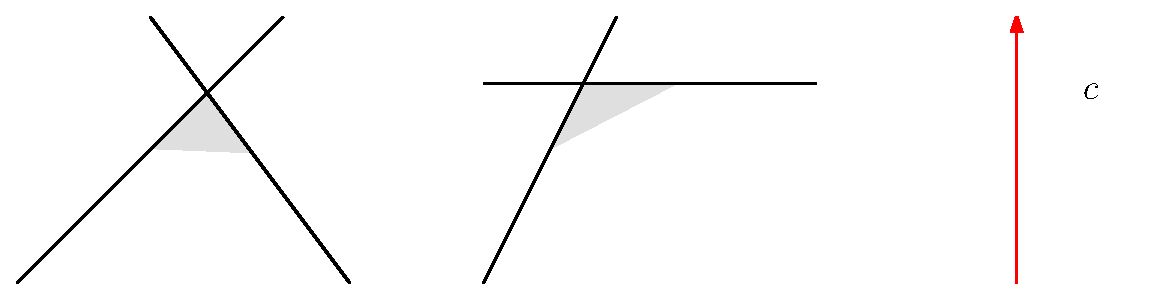
\epsfig{file=figures/degnodeg.eps,height=3cm}
  \caption{A non-degenerate and a degenerate roof}
  \label{fig:non-deg-deg}
\end{figure}





\begin{figure}[htbp]
  \centering
  {
    \psfrag{HPLR}{Optimum solution  and lowest roof}
    \psfrag{R}{A roof}
    \psfrag{N}{Not a roof}
    \psfrag{c}{$c$}
  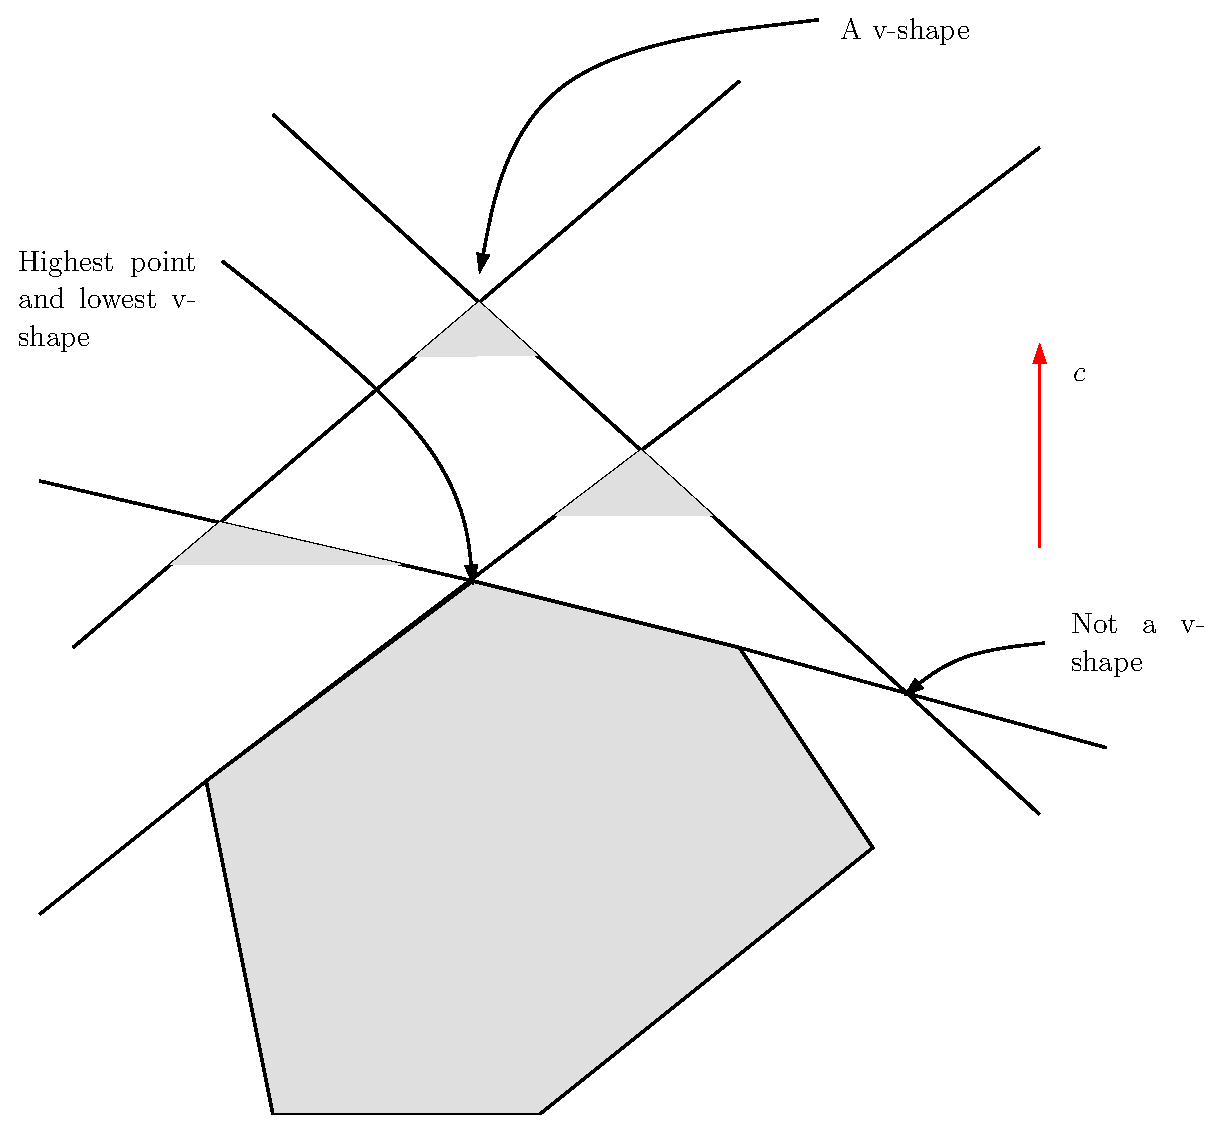
\epsfig{file=figures/highest_point.eps,height=10cm}
}
  \caption{Roofs and the optimum solution of a linear program}
  \label{fig:highest_point}
\end{figure}




\begin{theorem}[Weak duality]
  \label{thr:1}
  Let  $\er$ be a roof,  $x^*$ be a feasible point of the linear
  program and $y^*$ be an optimal solution of $\max\{c^Tx \colon x \in
  \setR^n, \, A_\er x \leq b_\er\}$, then $c^Tx^* \leq c^Ty^*$. 
\end{theorem}


\begin{proof}
  The point $x^*$ satisfies $Ax\leq b$ and thus $A_\er x\leq b_\er$. Since
  $y^*$ is an optimal solution of the linear program $\max\{c^Tx \colon x
  \in \setR^n, \, A_\er x \leq b_\er \}$,   the claim follows. 
\qed
\end{proof}


%In other words, the lowest roof is an upper bound on the highest
%point. 


%\begin{definition}[Conic combination, cone]
%  Let $S = \{a_1,\ldots,a_m\}$ be a set of vectors of $\setR^n$. 
%  A point 
%  \begin{displaymath}
%    v = \sum_{i=1}^m y(i) a_i 
%  \end{displaymath}
%  with $y \in \setR^m_{\geq0}$  is called a
%  \emph{conic combination} $S$. The conic
%  combination is \emph{strictly positive}, if each $y(i)>0$. 
%  The \emph{cone} generated by
%  $S$ is the set of all conic combinations of $S$, 
%  \begin{displaymath}
%    \ec(S) = \{ \sum_{i=1}^m y(i) a_i \mid y \in \setR^m, \, y\geq0\}.
%  \end{displaymath}
%\end{definition}





%\begin{figure}[htbp]
%  \centering
%  {
%    \psfrag{0}{$0$}
%    \psfrag{a1}{$a_1$}
%    \psfrag{a2}{$a_2$}
%    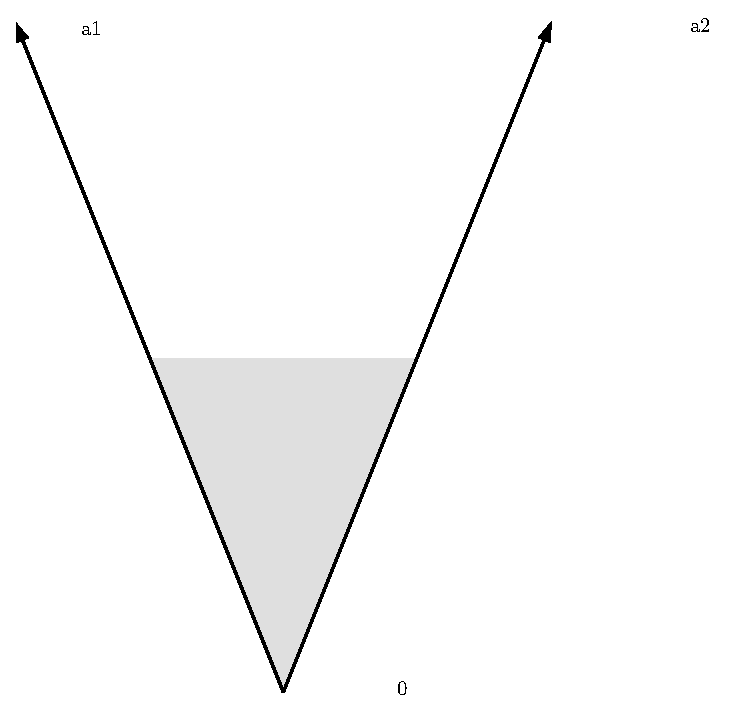
\epsfig{file=figures/cone.eps,height=3cm}
%}
%  \caption{The  cone generated by $a_1$ and $a_2$.}
%\label{fig:cone}
%\end{figure}



Next we give a characterization of roofs in terms of the objective
function vector being a conic combination of the rows of $A_\er$. 
\begin{lemma}
  \label{lem:4}
  The set $\er\subseteq\{1,\ldots,m\}$  is a roof
  if and only if  $|\er| =n$, $a_i, i \in \er$  are linearly independent and
  $c \in \cone(\{a_i\colon i \in \er\})$. 
\end{lemma}

\begin{proof}
  Suppose the condition holds. The unique solution $x^*$  to the
  system 
  \begin{equation}
    \label{eq:0}
    A_\er x = b_\er 
  \end{equation}
  is an optimal solution to
  $\hpp(\er,c)$. Because if $\wt{x}$ is another feasible solution,
  then $c^T\wt{x} = \sum_{i=1}^n y(i)a_i^T \wt{x}$. Since $y \geq0$ and
  $a_i^T\wt{x}\leq\beta_i$  we can write
  \begin{eqnarray}
    \label{eq:2}
    c^T\wt{x} & = &  \sum_{i=1}^n y(i)a_i^T  \wt{x}\\
             & \leq & \sum_{i=1}^n y(i) \beta_i \\
             & = &  \sum_{i=1}^n y(i) a_i^Tx^*\\
             & = & c^Tx^*.
  \end{eqnarray}
   Thus $\er$ is a roof. 

  Suppose on the other hand that $\er$ is a roof. Then, since
  $a_1,\ldots,a_n$ is a basis of $\setR^n$, there exists a $y\in \setR^n$ with 
  $c =  y(1)a_1+\ldots+y(n)a_n$. 
  
  Suppose that a component of $y$ is negative. Without loss of
  generality assume  $y(1)<0$. Consider the system of linear equations
  \begin{equation}
    \label{eq:1}
    a_1^Tx = -1,a_2^Tx=0,\ldots,a_n^Tx = 0.
  \end{equation}
  This system~\eqref{eq:1} has a unique solution $0\neq v\in \setR^n$.  
  Let $x^*$ be feasible for $\er$. Clearly $x^* + \lambda v$ is also feasible for each
  $\lambda>0$. But $c^T (x^* + \lambda v) = c^Tx^* + \sum_{i=1}^n y(i) \lambda a_i^T  v = c^T x^*
  + y(1)\lambda  a_1^Tv$. This increases with $\lambda$ since $y(1)<0$ and
  $a_1^Tv<0$.  This contradicts the fact that $\hpp(\er,c)$ is
  bounded. 
\qed 
\end{proof}



\begin{definition}
  \label{def:5}
  Let $\er = \{a_1^Tx\leq\beta_1,\ldots,a_n^Tx\leq\beta_n\}$ be a roof of
  $\hpp(\eh,c)$. The unique point $x^*$  which is a solution to the
  system 
  \begin{equation}
    \label{eq:3}
    a_1^Tx=\beta_1,\ldots,a_n^Tx=\beta_n
  \end{equation}
  is called the \emph{vertex} of $\er$. 
\end{definition}


The proof of Lemma~\ref{lem:4} reveals the following fact. 

\begin{proposition}
\label{prop:1}
Let $\er$ be a roof of $\hpp(\eh,c)$. The vertex of $\er$ is an
optimal solution to $\hpp(\er,c)$.
\end{proposition}


Similarly one can prove the following fact. 

\begin{proposition}
  \label{prop:2}
    The vertex of a   roof $\er = \{a_1^Tx\leq\beta_1,\ldots,a_n^Tx\leq\beta_n\}$   of $\hpp(\eh,c)$ 
    is the unique optimal solution of $\hpp(\er,c)$ if and only 
    if $c$ is a strictly positive conic combination  of 
    the normal-vectors $a_1,\ldots,a_n$. 
\end{proposition}

\begin{proof}
  Exercise.
\end{proof}


\begin{exercise}
  \label{sec:high-point-probl}
  Let $\er$ be a roof of $\hpp(\eh,c)$ with vertex $x^*$. Prove
  that the set of  feasible points of $\er$ is of the form 
  $x^* + \ec$, where $\ec$ is a cone. 
\end{exercise}


\section{The simplex algorithm}
\label{sec:simplex-algorithm}



Our goal is to prove  a strong version of Theorem~\ref{thr:1}. 

\begin{theorem}[Strong duality]
  \label{thr:5}
  If $\hpp(\eh,c)$ has an optimal solution, then there exists a
  roof whose vertex is an optimal solution to $\hpp(\eh,c)$. 
\end{theorem}
Figure~\ref{fig:highest_point} suggests that the theorem holds in the
plane. In the following we provide a proof for any dimension~$n$. For
this we assume that there exists a roof. This is legitimate for the
following reason. If $x^*$ is an optimal solution to $\hpp(\eh,c)$
then we can add the inequality $c^Tx \leq c^Tx^*+1$. Then we can easily
form a degenerate roof which contains this halfspace. Yet, this
halfspace can never be a part of the roof we are looking for, since
a vertex $\wt{x}$  of a roof which contains $c^Tx \leq c^Tx^*+1$  has
objective function $c^Tx^*+1$ which is too large. 

\subsection{The non-degenerate case}
\label{sec:non-degenerate-case}

Throughout this section assume that  $\hpp(\eh,c)$ is non-degenerate. 
We now describe a way to move from a given roof $\er$ to another
one. The outcome of this move will be one of the following.
%\begin{theorem}
%  \label{thr:2}
%  Let $\hpp(\eh,c)$ be a  highest point problem and suppose
%  that there exists a roof of $\hpp(\eh,c)$.  If $\eh$ is feasible,
%  then there exists a roof whose vertex is an optimal solution to
%  $\hpp(\eh,c)$. If $\eh$ is not feasible, then there exists a roof
%  $\ev$ and a halfspace $h \in \eh$ such that $\ev + h$ is infeasible. 
%\end{theorem}
%%
\begin{enumerate}
\item We can assert  that  the vertex $x^*$ of $\er$ is feasible for $\eh$ and
  thus an optimal  solution of $\hpp(\eh,c)$.  
\item We have a roof $\er'$ which is strictly lower than $\er$.
\item We can prove that $\eh$ is infeasible.
\end{enumerate}

\begin{figure}[htbp]
  \centering
  \epsfig{file=figures/entering.eps,height=5cm}
  \caption{On the left: A strictly lower roof. On the right: $\eh$
    is infeasible}
  \label{fig:two-poss}
\end{figure}


We now describe the procedure for this move. Suppose that $a_1,\ldots,a_n$
are the normal-vectors of the initial roof $\er$.

\noindent 
{\bf Step 1:}  Compute the vertex $x^*$ of $\er$. 

\begin{lemma}
  \label{lem:5}
  If there exists no halfspace $h \in \eh$ which is violated by $x^*$,
  then $x^*$ is an optimal solution to the highest point problem. 
\end{lemma}

\begin{proof}
  Easy!
\end{proof}

\noindent
{\bf Step 2:} Find a halfspace $a^Tx\leq\beta$ for which $x^*$ is not
feasible. If such a halfspace does not exist, then $\er$ is a lowest
roof and we stop.   


Let $a^Tx\leq\beta \in \eh$ with $a^T x^* > \beta$.  Our
goal is now to construct a new roof $\er'$ which is made up of
$n-1$~halfspaces of $\er$ and this new one $a^Tx\leq\beta$.  From
Lemma~\ref{lem:4} we have to represent $c$ as a nonnegative linear
combination of $a$ and some $n-1$~normal-vectors of $\er$.  

Consider the systems of equations 
\begin{eqnarray}
  a_1 y(1) + \ldots + a_n y(n) + a y(n+1) & = &  c \label{eq:5}\\
  a_1 v(1) + \ldots + a_n v(n) + a v(n+1) & = &  0. \label{eq:17}
\end{eqnarray}

\noindent
{\bf Step 3:} Compute  a  solution $y^* \in \setR^{n+1}$ of~\eqref{eq:5} with
last component $0$ and compute  solution $v^* \in \setR^{n+1}$
of~\eqref{eq:17} with last component $1$. The solutions
to~\eqref{eq:5} are the points on the line 
$\{ y^* + \lambda v^* \mid \lambda \in\setR\}$. 

To bring $a^Tx\leq\beta$ into the roof, we want to increase the last component 
until some other component, component $\ell$ lets say,  becomes zero.
The new roof is then $\er'=\er - \{a_\ell^Tx\leq\beta_\ell\} + \{a^Tx\leq\beta\}$. 

So in virtue of finding the halfspace which drops out of $\er$, we
have to determine the largest $\lambda^* \in \setR_{\geq0}$ such that all components of
$y^* + \lambda\,v^*$ are nonnegative. This is very simple. 

\noindent 
{\bf Step 4:} Compute   the index set $I \subseteq\{1,\ldots,n\}$ such that
$v^*(i)<0$. Those are the 
indices we have to worry about, since only those components of the
line can become negative with increasing $\lambda$. Still, how large can
$\lambda^*$ be? We have to ensure that
\begin{equation}
  \label{eq:8}
  y^*(i) +\lambda^* v^*(i) \geq0 \text{ for all } i \in I.
\end{equation}
In other words we have to ensure 
\begin{equation}
  \label{eq:4}
  \lambda^* \leq - \frac{y^*(i)}{v^*(i)} \text{ for all }  i\in I.
\end{equation}


\noindent 
{\bf If $I \neq \emptyset$: }

We pick 
 \begin{equation}
   \label{eq:9}
   \lambda^* = \min_{\substack{i\in I}}  - \frac{y^*(i)}{v^*(i)}. 
\end{equation}
There is exactly one index in $I$ for which this minimum is achieved
because $\hpp(\eh,c)$ is non-degenerate.  This unique index $\ell$ is the
one which leaves the roof.

\begin{lemma}
  \label{lem:1}
  The so found set of halfspaces  $\er' = \er - (a_\ell^Tx\leq\beta_\ell) +
  (a^Tx\leq\beta)$ is a roof. 
\end{lemma}
\begin{proof}
  We have already seen that $c$ is a nonnegative linear combination of
  the normal vectors of this set. Thus we only need to show that
  $\er'$ is linearly independent. This is very easy. If $\ell$ leaves
  $\er$, then $v^*(\ell)$ is nonzero. Since $v^*$ is a solution of
  equation~(\ref{eq:17}) it follows that $a_\ell$ is a linear combination
  of the normal-vectors of $\er'$. Thus $\er'$ is linearly
  independent. 
\qed
\end{proof}

With the next proposition, we show that the move from $\er$ to $\er'$
brings us closer to the lowest roof. Remember that the unique
optimum solution to $\hpp(\er,c)$ is the vertex of $\er$. Thus the
next proposition shows that the vertex of $\er'$ has a strictly
smaller objective value. 


\begin{proposition}
  \label{prop:3}
  The vertex $x'$ of $\er'$ is a feasible point of $\er$.
\end{proposition}

\begin{proof}
  Without loss of generality assume that $\ell =1$. 
  Let $x^*$ be the vertex of $\er$ and let $w \in \setR^n$ be a solution to
  the system 
  \begin{equation}
    \label{eq:15}
    a_1^Tx = -1, a_2^Tx=0,\ldots,a_n^Tx = 0.
  \end{equation}
  The halfline $l(x^*,w) = \{ x^* + \lambda \, w \mid \lambda \in \setR_{\geq0}\}$  is feasible
  for $\er$. We have the equation
  \begin{equation}
    \label{eq:16}
    a = -a_1v^*(1) - \ldots - a_nv^*(n),
  \end{equation}
  where $v^*(\ell) < 0$.  Thus 
  \begin{eqnarray}
    a^T w  & = & - \sum_{i=1}^n v^*(i) a_i^T w \\
          & = &  v^*(\ell) \\
          & < & 0.
  \end{eqnarray}
  Therefore the halfline  $l(x^*,w)$ enters at some point  $x'$ the
  halfspace $a^Tx\leq\beta$. This is the vertex $x'$ of $\er'$. 
\end{proof}

 \begin{figure}[htbp]
    \begin{center}
      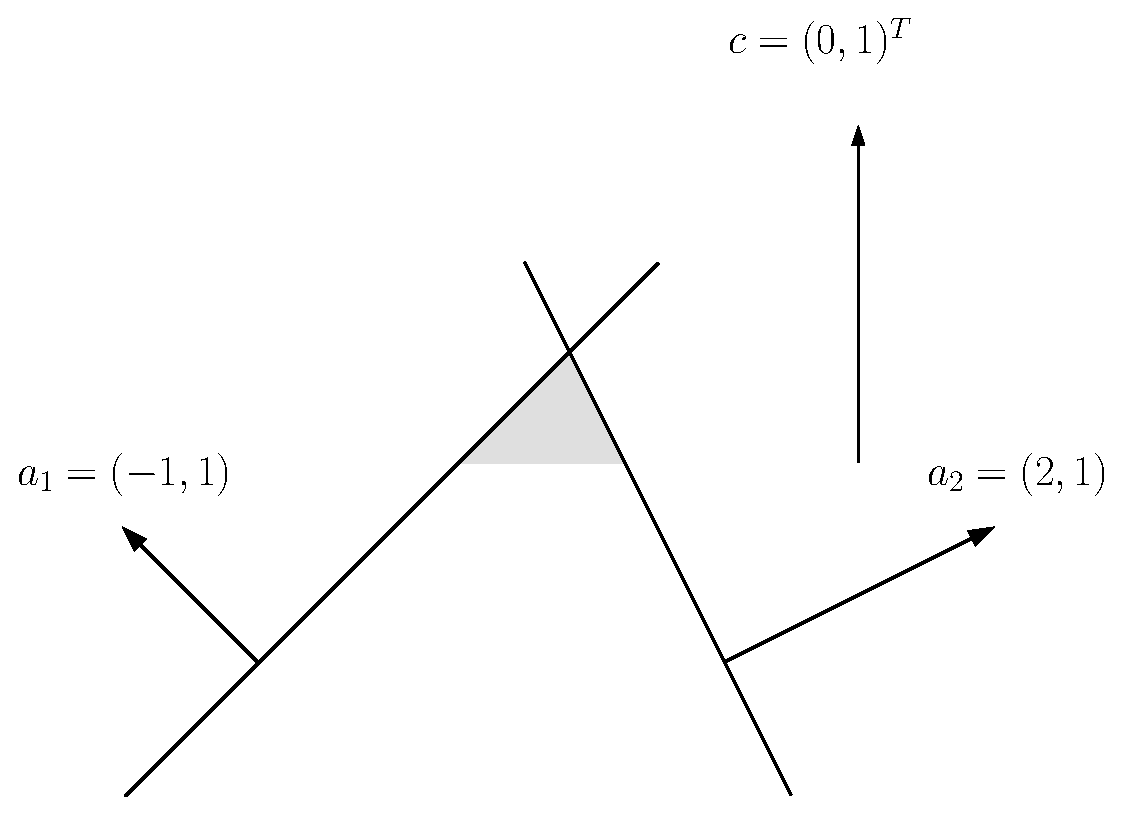
\epsfig{file=figures/example.eps,height=6cm}
      \caption{The initial roof  of Example~\ref{ex:1}.}
        \label{fig:ex:1.1}
    \end{center}    
  \end{figure}


\begin{example}
  \label{ex:1}
    
  Consider the roof $\er = \{(-1,1) x \leq 1, (2,1)x\leq1\}$ and suppose
  that $c = (0,1)^T$, see Figure~\ref{fig:ex:1.1}. Suppose that the
  halfspace $(1,2)x\leq1$ belongs to $\eh$. 
  
  \noindent 
  In step~1 we compute the vertex of $\er$ which is the solution to the
  system 
  \begin{equation}
    \label{eq:19}
    \mat{-1 & 1 \\ 2 & 1}  x  = \mat{1\\1}.
  \end{equation}
  By adding twice of the first row to the second row we obtain 
  \begin{equation}
    \label{eq:6}
     \mat{-1 & 1 \\ 0 & 3}  x  = \mat{1\\3},
  \end{equation}
  and we see that 
  the  vertex is the vector $x^* = \smat{0\\1}$.  
  
  \noindent 
  In step~2 we find that the halfspace $(1,2) x \leq1$ is not satisfied
  by $x^* = \smat{0\\1}$. We want to bring this halfspace into the new
  roof $\er'$.
  
  \noindent 
  Step~3:
  Now we compute the solution  to the system 
  \begin{equation}
    \label{eq:20}
    \mat{-1 & 2 \\ 1 & 1} y = \mat{0\\1}
  \end{equation}
  and  find $y^* = \smat{2/3 \\ 1/3 \\ 0}$.  
  
  Next we find a solution  to the system 
   \begin{equation}
     \label{eq:21}
    \mat{-1 & 2 \\ 1 & 1} \mat{v(1) \\ v(2)} = - \mat{1\\2}
  \end{equation} 
  and find  $v^* = \smat{-1\\ - 1 \\ 1}$. 
  
  \noindent
  The index set $I = \{1,2\}$ is not empty. The minimum~\eqref{eq:9} is
  achieved at  $\ell =2$. So the halfspace 
  $(2,1)x\leq1$ will leave the roof. Thus $\er'$ is
  the roof $\{(-1,1)x \leq 1,
  (1,2)x\leq1\}$.  This is also what we immediately see by
  looking at Figure~\ref{fig:ex:1.2}. 
   
\end{example}

  \begin{figure}[htbp]
    \begin{center}
      
      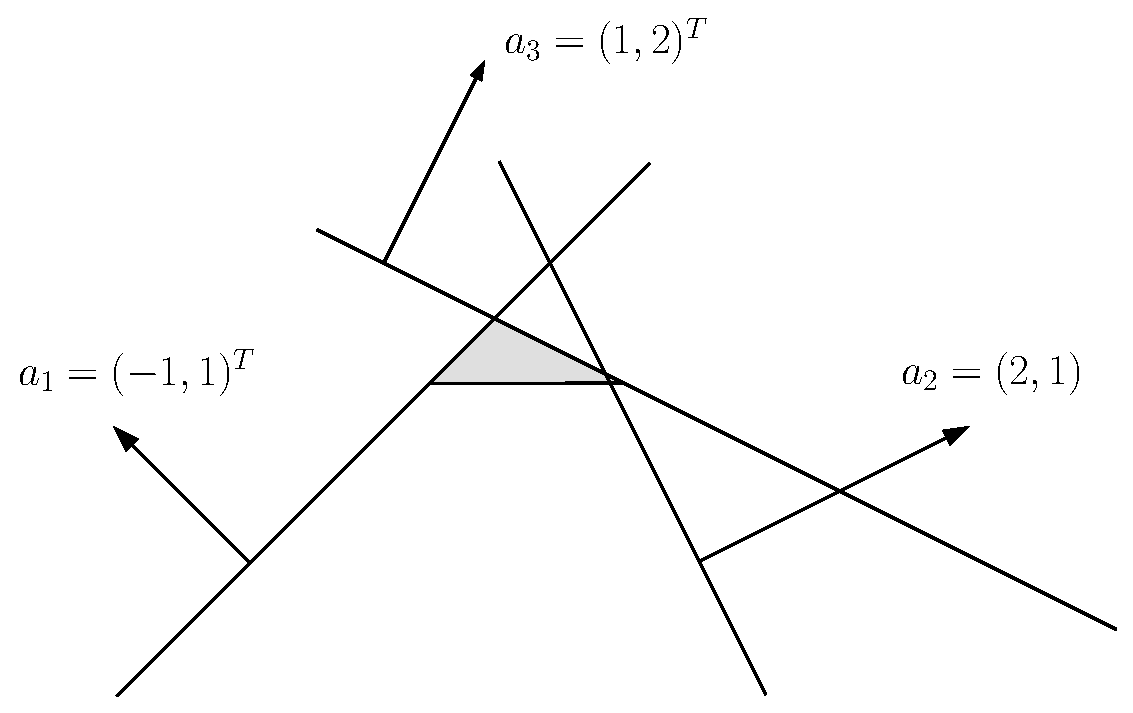
\epsfig{file=figures/example2.eps,height=6cm} 
      \caption{The new roof from  Example~\ref{ex:1}.} 
      \label{fig:ex:1.2}
    \end{center}
  \end{figure}


\noindent 
{\bf If $I = \emptyset$: } We assert that $\hpp(\eh,c)$ is infeasible based on
the following result. 

\begin{proposition}
  \label{thr:3}
  The set of halfspaces   $\er + (a^Tx \leq\beta)$ is infeasible if and only
  if $I = \emptyset$.
\end{proposition}

\begin{proof}
  The index set  $I$ is empty if and only if $v^*\geq0$. Let $\wt{x}$ be
  feasible for $\er$. We now 
  show that $\wt{x}$ is not feasible for $a^Tx\leq\beta$. The assertion then
  follows, because  $\er + (a^Tx\leq\beta) \subseteq \eh$. 
  For this we need to show that $a^T\wt{x}>\beta$, or equivalently 
  $-a^T\wt{x} < -\beta$.  
  
  Just let the formalism work for you. In the following equations,
  $x^*$ stands for the vertex of $\er$. Remember, that $x^*$ does not
  satisfy $a^Tx\leq\beta$. 

  \begin{eqnarray}
    -a^T \wt{x} & = & \left( a_1 v^*(1) + \ldots + a_n v^*(n)\right)^T  \wt{x} \label{eq:10}\\
               & = & \sum_{i=1}^n v^*(i) a_i^T\wt{x} \label{eq:11}\\
               & \leq &  \sum_{i=1}^n v^*(i) a_i^T x^*  \label{eq:12}\\ 
               & = &  -a^T x^*   \label{eq:13}\\
               & < & - \beta. \label{eq:14}
  \end{eqnarray}
From~\eqref{eq:11} to~\eqref{eq:12} we have used the fact that
$v(i)\geq0$ and  $a_i^T\wt{x} \leq\beta_i$ and that $a_i^Tx^* = \beta_i$.
From~\eqref{eq:13} to~\eqref{eq:14} we only used that $a^Tx^* >
\beta$. 


Similarly we can see that, if a point $\wt{x}$ is feasible for all 
halfspaces in $\er$ and the halfspace $a^Tx\leq\beta$, then $v^*$ cannot be
positive. Because we proved above that $v^*\geq0$ implies that each
feasible point for $\er$ is infeasible for $a^Tx\leq\beta$. 
\end{proof}


This algorithm which we have just described is called
\emph{pivoting}. 
Now we can describe the famous simplex algorithm which finds the
lowest roof of a HPP. It simply keeps pivoting until one can
assert  that  $\eh$ is infeasible or unbounded or until a lowest
roof is found. 

\begin{algorithm}[Simplex]~\\
  \begin{tabular}{ll}
    {\bf Input:}  & non-degenerate $\hpp(\eh,c)$ and a roof $\er$\\
    {\bf Output:} & lowest roof $\er'$ \\
    & or assertion that $\eh$ is infeasible 
  \end{tabular}
  
  \begin{enumerate}
  \item $\wt{\er} \gets \er$
  \item {\bf REPEAT}
    \begin{enumerate}
    \item Run {\bf Pivot} on $\wt{\er}$
    \item If this reveals that $\wt{\er}$ is lowest roof
      \begin{enumerate}
      \item {\bf RETURN} $\wt{\er}$
      \end{enumerate}
    \item If this reveals that $\eh$ is infeasible
      \begin{enumerate}
      \item {\bf RETURN} $\eh$ is infeasible
      \end{enumerate}
    \item If this returns roof $\er'$ \label{item:2}
      \begin{enumerate}
      \item  $\wt{\er} \gets \er'$
      \end{enumerate}
    \end{enumerate}
    \item {\bf UNTIL} 0
  \end{enumerate}
\end{algorithm}


\begin{theorem}
  \label{thr:4}
  The simplex algorithm terminates after a finite number of steps on a
  non-degenerate HPP. 
\end{theorem}

\begin{proof}
  The only interesting step is~\ref{item:2}). The vertex of the new
  roof is feasible for the old roof by
  Proposition~\ref{prop:3}. Since the HPP is non-degenerate, this new
  vertex has a strictly smaller objective function. Since there are
  only a finite number of roofs, the simplex algorithm terminates. 
\end{proof}

This gives us also a proof of our strong duality theorem for
non-degenerate HPP's. 






\subsection{The degenerate case}
\label{sec:degenerate-case}

The termination argument for the non-degenerate case was that the
optimal value of the roof is strictly dropping and thus, that a
roof can never be revisited. Since there are only a finite number
of roofs, this implies that the simplex algorithm terminates.

In the degenerate case, roofs could be revisited. This phenomenon
is called \emph{cycling}. What can we do about it? Here we change the
objective vector $c \in \setR^n$ a little bit and turn it into a vector
$c_\epsilon$ such that the following conditions hold. 

\begin{enumerate}
\item The highest point problem $\hpp(\eh,c_\epsilon)$ has roofs.\label{item:1}
\item A roof of $\hpp(\eh,c_\epsilon)$ is a roof of $\hpp(\eh,c)$.\label{item:3}
\item No roof of $\hpp(\eh,c_\epsilon)$ is degenerate. \label{item:4}
\end{enumerate}


Suppose we have an initial roof
$\wt{\er}=\{\wt{a}_1^Tx\leq\beta_1,\ldots,\wt{a}_n^Tx\leq\beta_n\}$ at the beginning of the
simplex algorithm and let $\wt{A}\in \setR^{n\times n}$ be the matrix whose
columns are the normal-vectors of $\wt{\er}$,
$\wt{A}=\left(\wt{a}_1,\ldots,\wt{a}_n\right)$. The system $\wt{A} \,y =c$
has a solution $\wt{y}\geq0$, where some components of $\wt{y}$ could be equal
to zero. This is undesirable and we wish that $\wt{y}$ is replaced by
\begin{equation}
  \label{eq:7}
  \wt{y} +  \mat{\epsilon \\ \epsilon^2 \\ \vdots \\\epsilon^n}
\end{equation}
for some $\epsilon>0$. Later it will
become clear why we add the vector $(\epsilon,\ldots,\epsilon^n)^T$ instead of the vector
$(\epsilon,\ldots,\epsilon)^T$. Now the vector~\eqref{eq:7} becomes a solution if we
perturb $c$ and consider the vector 
\begin{equation}
  \label{eq:18}
  c_\epsilon = c + \wt{A} \mat{\epsilon \\ \epsilon^2 \\ \vdots \\\epsilon^n}
\end{equation}
instead. If $\epsilon>0$, then $\wt{\er}$ is a non-degenerate roof of
$\hpp(\eh,c_\epsilon)$. Thus condition~\ref{item:1}) holds for any $\epsilon>0$. In
the sequel, we make $\epsilon$ smaller and smaller, such that also the
conditions~\ref{item:3}) and~\ref{item:4}) will be satisfied. 

Let us  first deal with condition~\ref{item:3}). Let 
$\eu=\{a_1^Tx\leq\beta_1,\ldots,a_n^Tx\leq\beta_n\}\subseteq\eh$ be a set of linear independent
halfspaces, which is not a roof of $\hpp(\eh,c)$. 
Let $A \in R^{n\times n}$ be the matrix $A = (a_1,\ldots,a_n)$. 
Since $\eu$ is not a roof, the vector $A^{-1}\,c $ has a strictly
negative component. Suppose that this component is the $i$-th
component $(A^{-1}\,c)(i)<0$.  By choosing $\epsilon>0$ sufficiently small,
we guarantee that   
\begin{eqnarray}
  (A^{-1}\,c_\epsilon)(i) & = & (A^{-1}\, c + A^{-1}\wt{A} \mat{\epsilon \\ \epsilon^2 \\ \vdots \\\epsilon^n})(i)\label{eq:23}\\
                & < & 0. 
\end{eqnarray}
Thus condition~\ref{item:3} is satisfied by choosing $\epsilon>0$
sufficiently small. 

For  condition~\ref{item:4} we have to work only a little harder, and
in fact, this is why we add the vector $(\epsilon,\ldots,\epsilon^n)$ instead of
$(\epsilon,\ldots,\epsilon)$. Let $\er$ be a roof of $\hpp(\eh,c)$ with normal vectors
$a_1,\ldots,a_n$ and let $A \in \setR^{n\times n}$ be again the matrix $A=(a_1,\ldots,a_n)$.
We now argue that, if  $\epsilon$ is sufficiently small, then $A^{-1}c_\epsilon$
does not have any component equal to  zero.  We are done then in
showing that, for $\epsilon$ sufficiently small, $\hpp(\eh,c_\epsilon)$ is
non-degenerate. Because any roof of $\hpp(\eh,c_\epsilon)$ will then be
non-degenerate. 

So let us inspect the vector 
\begin{equation}
  \label{eq:24}
  A^{-1} c_\epsilon = A^{-1}c + A^{-1}\cdot \wt{A} \mat{\epsilon \\ \vdots \\ \epsilon^n}. 
\end{equation}
Each component of \eqref{eq:24} is a nonzero polynomial with
variable~$\epsilon$.  Nonzero, because $A$ and $\wt{A}$ are non-singular
matrices. It is well known, that a nonzero polynomial of degree~$n$
has at most $n$ roots. Thus, for $\epsilon>0$, sufficiently  small, no
component of~\eqref{eq:24} will be zero. 



So the conditions~\ref{item:1}), \ref{item:3}) and \ref{item:4}) hold
for $\epsilon>0$ sufficiently small. Thus we can modify a degenerate HPP into
a non-degenerate HPP and apply the simplex algorithm to it. Thus we
obtain a proof of the strong duality theorem. 

\subsection{The lexicographic pivot rule}
\label{sec:lexic-pivot-rule}


We now show that we do not have to physically perform the
perturbation which sends $c$ to $c_\epsilon$, but instead describe a rule to
choose the leaving roof from the possible candidates for which the
minimum in~(\ref{eq:9}) is attained. Rules for entering and exiting
roofs are called \emph{pivoting rules}.  


So let us inspect step~3 for the perturbed problem
$\hpp(\eh,c_\epsilon)$. The solution $v^*$ to~(\ref{eq:17}) is the same for
the perturbed and non-perturbed problem. However, the solution
to~(\ref{eq:5})  is equal to 
\begin{equation}
  \label{eq:25}
  y^* + A^{-1} \cdot \wt{A} \mat{\epsilon \\ \vdots \\ \epsilon^n},
\end{equation}
where we neglect the last zero component. 
Now again, let $I \subseteq\{1,\ldots,n\}$ be the in $v^*(i)<0$. In the perturbed
problem, we determine the index $\ell \in I$ such that 
\begin{equation}
  \label{eq:26}
  - (y^*(\ell) + A^{-1} \cdot \wt{A} \mat{\epsilon \\ \vdots \\ \epsilon^n})(\ell) / v^*(\ell) 
\end{equation}
is minimal. In the unperturbed problem, there could be a set $L\subseteq I$ of
indices, for which the minimum is attained. 

\begin{definition}[Lexicographic order, $\geq_{\lex}$]
  \label{def:2}
  Let $u$ and $v$ be vectors of $\setR^n$. We say that $u\geq_{\lex}v$ if the
  first nonzero entry of $u-v$ is positive. We say that $u$ is
  \emph{lexicographically larger} than $v$. If $u \neq v$ then we write $u>_{\lex}v$. 
\end{definition}
%
In the following we write $r_j(\epsilon)$ for the $j$-th polynomial  
\begin{equation}
  \label{eq:27}
  -(y^*(j) + A^{-1} \cdot \wt{A} \mat{\epsilon \\ \vdots \\ \epsilon^n})(j) / v^*(j), \, j \in L.
\end{equation}
%
This polynomial is defined by its coefficient vector $r_j\in
\setR^{n+1}$.  The vector $r_j$ is the $j$-th row of the matrix 
$- \left( y^*, A^{-1} \cdot \wt{A}\right)$ divided by $v^*(j)$. 
We imitate the perturbed choice by choosing the index $\ell$ such that 
$r_j$ is lexicographically smallest. 
Let us spend a little more time in explaining why.  Let $r_\ell$
be this lexicographically smallest vector. Since $ A^{-1} \cdot \wt{A}$ is
non-singular, each row $r_j$ is strictly larger than $r_\ell$. 
This means that $r_j - r_\ell$ is a vector whose first nonzero component
is strictly positive. Thus $(r_j - r_\ell)(\epsilon) >0$ for $\epsilon$ sufficiently
small. 


Thus the following lexicographic  pivoting rule guarantees the
termination of the simplex method. 

\begin{itemize}
\item   Determine the set $L\subseteq I$ for which the minimum 
  \begin{displaymath}
    \min_{i \in I} -  y^*(i)/v^*(i)
  \end{displaymath}
  is attained.  
  \item Choose the index $\ell \in L$  such that 
  \begin{displaymath}
    \frac{\ell\mbox{-th row} - \left( y^*, A^{-1}\cdot\wt{A}\right)}{v^*(\ell)} \leq_\lex 
    \frac{j\mbox{-th row} - \left( y^*, A^{-1} \cdot \wt{A}\right)}{v^*(j)} \mbox{ for each } j \in L.
  \end{displaymath}
  \item The $\ell$-th halfspace leaves the roof. 
\end{itemize}



\section{Phase~I, finding an initial roof}
\label{sec:phase-i-finding}


So far, we always started with an initial roof. Where do we get 
it  from?  This is where Phase~I of the simplex method is put to
work. 

{\bf Step 1:} Form an auxiliary HPP, $\hpp{\eh',c}$, where $\eh'$
consists of the halfspaces $a^Tx\leq0$ for each halfspace $a^Tx \leq \beta \in\eh$ 

together with the halfspaces 
\begin{equation}
  \label{eq:22}
  \begin{array}{ll}
    x(i) \leq 1 & \mbox{ for } c(i)\geq0,\\
    -x(i)\leq 1 & \mbox{ for } c(i)<0. 
  \end{array}
\end{equation}

Notice that $\hpp{\eh',c}$ is feasible and has a roof $\er$, namely
the inequalities~(\ref{eq:22}).  The vertex $x^*$ of each roof,
which contains one of the inequalities~\eqref{eq:22} has a positive
objective value $c^Tx^*$. On the other hand, a roof of
$\hpp(\eh,c)$ yields a roof of $\hpp{\eh',c}$ with vertex $x^*=0$.
We start the simplex algorithm on this auxiliary HPP. If we obtain a
roof with vertex $x^*$ such that $c^Tx^*>0$, then the original
$\hpp(\eh,c)$ does not contain roofs. Otherwise, we have identified
a set of linear independent halfspaces $\eu \subseteq\eh$ such that $c$ is a
conic combination of the normal-vectors of $\eu$. If $|\eu|<n$,  we complete
$\eu$ to a degenerate roof $\er$ of $\hpp(\eh,c)$. Otherwise $\eu$
is already a roof. 


\section{The running time of the simplex method}
\label{sec:running-time-simplex}


Starting at a roof $\er$, it may happen, that one basically visits
all roofs of $\hpp(\eh,c)$ before one arrives at the lowest
roof. The number of roofs is bounded by $\binom{m}{n} =
\bigO(m^n)$. This is {\bf exponential} in the dimension. Thus the
simplex algorithm runs in polynomial time if the dimension is
fixed. We will see later, that there exists an algorithm, which solves
the highest point problem in polynomial time, even if the dimension
varies. 

However, the simplex method performs very well in practice. 



%%% Local Variables: 
%%% mode: latex
%%% TeX-master: "lecture"
%%% End: 
